% TODO
% mention lossless <- simplifies...
% example of need of virt channels
% more topologies





%% bare_conf.tex
%% V1.3
%% 2007/01/11
%% by Michael Shell
%% See:
%% http://www.michaelshell.org/
%% for current contact information.
%%
%% This is a skeleton file demonstrating the use of IEEEtran.cls
%% (requires IEEEtran.cls version 1.7 or later) with an IEEE conference paper.
%%
%% Support sites:
%% http://www.michaelshell.org/tex/ieeetran/
%% http://www.ctan.org/tex-archive/macros/latex/contrib/IEEEtran/
%% and
%% http://www.ieee.org/

%%*************************************************************************
%% Legal Notice:
%% This code is offered as-is without any warranty either expressed or
%% implied; without even the implied warranty of MERCHANTABILITY or
%% FITNESS FOR A PARTICULAR PURPOSE! 
%% User assumes all risk.
%% In no event shall IEEE or any contributor to this code be liable for
%% any damages or losses, including, but not limited to, incidental,
%% consequential, or any other damages, resulting from the use or misuse
%% of any information contained here.
%%
%% All comments are the opinions of their respective authors and are not
%% necessarily endorsed by the IEEE.
%%
%% This work is distributed under the LaTeX Project Public License (LPPL)
%% ( http://www.latex-project.org/ ) version 1.3, and may be freely used,
%% distributed and modified. A copy of the LPPL, version 1.3, is included
%% in the base LaTeX documentation of all distributions of LaTeX released
%% 2003/12/01 or later.
%% Retain all contribution notices and credits.
%% ** Modified files should be clearly indicated as such, including  **
%% ** renaming them and changing author support contact information. **
%%
%% File list of work: IEEEtran.cls, IEEEtran_HOWTO.pdf, bare_adv.tex,
%%                    bare_conf.tex, bare_jrnl.tex, bare_jrnl_compsoc.tex
%%*************************************************************************

% *** Authors should verify (and, if needed, correct) their LaTeX system  ***
% *** with the testflow diagnostic prior to trusting their LaTeX platform ***
% *** with production work. IEEE's font choices can trigger bugs that do  ***
% *** not appear when using other class files.                            ***
% The testflow support page is at:
% http://www.michaelshell.org/tex/testflow/



% Note that the a4paper option is mainly intended so that authors in
% countries using A4 can easily print to A4 and see how their papers will
% look in print - the typesetting of the document will not typically be
% affected with changes in paper size (but the bottom and side margins will).
% Use the testflow package mentioned above to verify correct handling of
% both paper sizes by the user's LaTeX system.
%
% Also note that the "draftcls" or "draftclsnofoot", not "draft", option
% should be used if it is desired that the figures are to be displayed in
% draft mode.
%
\documentclass[conference]{IEEEtran}
% Add the compsoc option for Computer Society conferences.
%
% If IEEEtran.cls has not been installed into the LaTeX system files,
% manually specify the path to it like:
% \documentclass[conference]{../sty/IEEEtran}





% Some very useful LaTeX packages include:
% (uncomment the ones you want to load)


% *** MISC UTILITY PACKAGES ***
%
%\usepackage{ifpdf}
% Heiko Oberdiek's ifpdf.sty is very useful if you need conditional
% compilation based on whether the output is pdf or dvi.
% usage:
% \ifpdf
%   % pdf code
% \else
%   % dvi code
% \fi
% The latest version of ifpdf.sty can be obtained from:
% http://www.ctan.org/tex-archive/macros/latex/contrib/oberdiek/
% Also, note that IEEEtran.cls V1.7 and later provides a builtin
% \ifCLASSINFOpdf conditional that works the same way.
% When switching from latex to pdflatex and vice-versa, the compiler may
% have to be run twice to clear warning/error messages.






% *** CITATION PACKAGES ***
%
%\usepackage{cite}
% cite.sty was written by Donald Arseneau
% V1.6 and later of IEEEtran pre-defines the format of the cite.sty package
% \cite{} output to follow that of IEEE. Loading the cite package will
% result in citation numbers being automatically sorted and properly
% "compressed/ranged". e.g., [1], [9], [2], [7], [5], [6] without using
% cite.sty will become [1], [2], [5]--[7], [9] using cite.sty. cite.sty's
% \cite will automatically add leading space, if needed. Use cite.sty's
% noadjust option (cite.sty V3.8 and later) if you want to turn this off.
% cite.sty is already installed on most LaTeX systems. Be sure and use
% version 4.0 (2003-05-27) and later if using hyperref.sty. cite.sty does
% not currently provide for hyperlinked citations.
% The latest version can be obtained at:
% http://www.ctan.org/tex-archive/macros/latex/contrib/cite/
% The documentation is contained in the cite.sty file itself.






% *** GRAPHICS RELATED PACKAGES ***
%
\ifCLASSINFOpdf
  \usepackage[pdftex]{graphicx}
  % declare the path(s) where your graphic files are
  % \graphicspath{{../pdf/}{../jpeg/}}
  % and their extensions so you won't have to specify these with
  % every instance of \includegraphics
  % \DeclareGraphicsExtensions{.pdf,.jpeg,.png}
\else
  % or other class option (dvipsone, dvipdf, if not using dvips). graphicx
  % will default to the driver specified in the system graphics.cfg if no
  % driver is specified.
  % \usepackage[dvips]{graphicx}
  % declare the path(s) where your graphic files are
  % \graphicspath{{../eps/}}
  % and their extensions so you won't have to specify these with
  % every instance of \includegraphics
  % \DeclareGraphicsExtensions{.eps}
\fi
% graphicx was written by David Carlisle and Sebastian Rahtz. It is
% required if you want graphics, photos, etc. graphicx.sty is already
% installed on most LaTeX systems. The latest version and documentation can
% be obtained at: 
% http://www.ctan.org/tex-archive/macros/latex/required/graphics/
% Another good source of documentation is "Using Imported Graphics in
% LaTeX2e" by Keith Reckdahl which can be found as epslatex.ps or
% epslatex.pdf at: http://www.ctan.org/tex-archive/info/
%
% latex, and pdflatex in dvi mode, support graphics in encapsulated
% postscript (.eps) format. pdflatex in pdf mode supports graphics
% in .pdf, .jpeg, .png and .mps (metapost) formats. Users should ensure
% that all non-photo figures use a vector format (.eps, .pdf, .mps) and
% not a bitmapped formats (.jpeg, .png). IEEE frowns on bitmapped formats
% which can result in "jaggedy"/blurry rendering of lines and letters as
% well as large increases in file sizes.
%
% You can find documentation about the pdfTeX application at:
% http://www.tug.org/applications/pdftex





% *** MATH PACKAGES ***
%
%\usepackage[cmex10]{amsmath}
% A popular package from the American Mathematical Society that provides
% many useful and powerful commands for dealing with mathematics. If using
% it, be sure to load this package with the cmex10 option to ensure that
% only type 1 fonts will utilized at all point sizes. Without this option,
% it is possible that some math symbols, particularly those within
% footnotes, will be rendered in bitmap form which will result in a
% document that can not be IEEE Xplore compliant!
%
% Also, note that the amsmath package sets \interdisplaylinepenalty to 10000
% thus preventing page breaks from occurring within multiline equations. Use:
%\interdisplaylinepenalty=2500
% after loading amsmath to restore such page breaks as IEEEtran.cls normally
% does. amsmath.sty is already installed on most LaTeX systems. The latest
% version and documentation can be obtained at:
% http://www.ctan.org/tex-archive/macros/latex/required/amslatex/math/





% *** SPECIALIZED LIST PACKAGES ***
%
%\usepackage{algorithmic}
% algorithmic.sty was written by Peter Williams and Rogerio Brito.
% This package provides an algorithmic environment fo describing algorithms.
% You can use the algorithmic environment in-text or within a figure
% environment to provide for a floating algorithm. Do NOT use the algorithm
% floating environment provided by algorithm.sty (by the same authors) or
% algorithm2e.sty (by Christophe Fiorio) as IEEE does not use dedicated
% algorithm float types and packages that provide these will not provide
% correct IEEE style captions. The latest version and documentation of
% algorithmic.sty can be obtained at:
% http://www.ctan.org/tex-archive/macros/latex/contrib/algorithms/
% There is also a support site at:
% http://algorithms.berlios.de/index.html
% Also of interest may be the (relatively newer and more customizable)
% algorithmicx.sty package by Szasz Janos:
% http://www.ctan.org/tex-archive/macros/latex/contrib/algorithmicx/




% *** ALIGNMENT PACKAGES ***
%
%\usepackage{array}
% Frank Mittelbach's and David Carlisle's array.sty patches and improves
% the standard LaTeX2e array and tabular environments to provide better
% appearance and additional user controls. As the default LaTeX2e table
% generation code is lacking to the point of almost being broken with
% respect to the quality of the end results, all users are strongly
% advised to use an enhanced (at the very least that provided by array.sty)
% set of table tools. array.sty is already installed on most systems. The
% latest version and documentation can be obtained at:
% http://www.ctan.org/tex-archive/macros/latex/required/tools/


%\usepackage{mdwmath}
%\usepackage{mdwtab}
% Also highly recommended is Mark Wooding's extremely powerful MDW tools,
% especially mdwmath.sty and mdwtab.sty which are used to format equations
% and tables, respectively. The MDWtools set is already installed on most
% LaTeX systems. The lastest version and documentation is available at:
% http://www.ctan.org/tex-archive/macros/latex/contrib/mdwtools/


% IEEEtran contains the IEEEeqnarray family of commands that can be used to
% generate multiline equations as well as matrices, tables, etc., of high
% quality.


%\usepackage{eqparbox}
% Also of notable interest is Scott Pakin's eqparbox package for creating
% (automatically sized) equal width boxes - aka "natural width parboxes".
% Available at:
% http://www.ctan.org/tex-archive/macros/latex/contrib/eqparbox/





% *** SUBFIGURE PACKAGES ***
%\usepackage[tight,footnotesize]{subfigure}
% subfigure.sty was written by Steven Douglas Cochran. This package makes it
% easy to put subfigures in your figures. e.g., "Figure 1a and 1b". For IEEE
% work, it is a good idea to load it with the tight package option to reduce
% the amount of white space around the subfigures. subfigure.sty is already
% installed on most LaTeX systems. The latest version and documentation can
% be obtained at:
% http://www.ctan.org/tex-archive/obsolete/macros/latex/contrib/subfigure/
% subfigure.sty has been superceeded by subfig.sty.



%\usepackage[caption=false]{caption}
\usepackage[font=footnotesize]{subfig}
% subfig.sty, also written by Steven Douglas Cochran, is the modern
% replacement for subfigure.sty. However, subfig.sty requires and
% automatically loads Axel Sommerfeldt's caption.sty which will override
% IEEEtran.cls handling of captions and this will result in nonIEEE style
% figure/table captions. To prevent this problem, be sure and preload
% caption.sty with its "caption=false" package option. This is will preserve
% IEEEtran.cls handing of captions. Version 1.3 (2005/06/28) and later 
% (recommended due to many improvements over 1.2) of subfig.sty supports
% the caption=false option directly:
%\usepackage[caption=false,font=footnotesize]{subfig}
%
% The latest version and documentation can be obtained at:
% http://www.ctan.org/tex-archive/macros/latex/contrib/subfig/
% The latest version and documentation of caption.sty can be obtained at:
% http://www.ctan.org/tex-archive/macros/latex/contrib/caption/




% *** FLOAT PACKAGES ***
%
%\usepackage{fixltx2e}
% fixltx2e, the successor to the earlier fix2col.sty, was written by
% Frank Mittelbach and David Carlisle. This package corrects a few problems
% in the LaTeX2e kernel, the most notable of which is that in current
% LaTeX2e releases, the ordering of single and double column floats is not
% guaranteed to be preserved. Thus, an unpatched LaTeX2e can allow a
% single column figure to be placed prior to an earlier double column
% figure. The latest version and documentation can be found at:
% http://www.ctan.org/tex-archive/macros/latex/base/



%\usepackage{stfloats}
% stfloats.sty was written by Sigitas Tolusis. This package gives LaTeX2e
% the ability to do double column floats at the bottom of the page as well
% as the top. (e.g., "\begin{figure*}[!b]" is not normally possible in
% LaTeX2e). It also provides a command:
%\fnbelowfloat
% to enable the placement of footnotes below bottom floats (the standard
% LaTeX2e kernel puts them above bottom floats). This is an invasive package
% which rewrites many portions of the LaTeX2e float routines. It may not work
% with other packages that modify the LaTeX2e float routines. The latest
% version and documentation can be obtained at:
% http://www.ctan.org/tex-archive/macros/latex/contrib/sttools/
% Documentation is contained in the stfloats.sty comments as well as in the
% presfull.pdf file. Do not use the stfloats baselinefloat ability as IEEE
% does not allow \baselineskip to stretch. Authors submitting work to the
% IEEE should note that IEEE rarely uses double column equations and
% that authors should try to avoid such use. Do not be tempted to use the
% cuted.sty or midfloat.sty packages (also by Sigitas Tolusis) as IEEE does
% not format its papers in such ways.





% *** PDF, URL AND HYPERLINK PACKAGES ***
%
%\usepackage{url}
% url.sty was written by Donald Arseneau. It provides better support for
% handling and breaking URLs. url.sty is already installed on most LaTeX
% systems. The latest version can be obtained at:
% http://www.ctan.org/tex-archive/macros/latex/contrib/misc/
% Read the url.sty source comments for usage information. Basically,
% \url{my_url_here}.





% *** Do not adjust lengths that control margins, column widths, etc. ***
% *** Do not use packages that alter fonts (such as pslatex).         ***
% There should be no need to do such things with IEEEtran.cls V1.6 and later.
% (Unless specifically asked to do so by the journal or conference you plan
% to submit to, of course. )


% correct bad hyphenation here
\hyphenation{op-tical net-works semi-conduc-tor}


\begin{document}
%
% paper title
% can use linebreaks \\ within to get better formatting as desired
\title{A Transport-Layer Network for Distributed FPGA Platforms}


% author names and affiliations
% use a multiple column layout for up to three different
% affiliations
%\author{\IEEEauthorblockN{Michael Shell}
%\IEEEauthorblockA{School of Electrical and\\Computer Engineering\\
%Georgia Institute of Technology\\
%Atlanta, Georgia 30332--0250\\
%Email: http://www.michaelshell.org/contact.html}
%\and
%\IEEEauthorblockN{Homer Simpson}
%\IEEEauthorblockA{Twentieth Century Fox\\
%Springfield, USA\\
%Email: homer@thesimpsons.com}
%\and
%\IEEEauthorblockN{James Kirk\\ and Montgomery Scott}
%\IEEEauthorblockA{Starfleet Academy\\
%San Francisco, California 96678-2391\\
%Telephone: (800) 555--1212\\
%Fax: (888) 555--1212}}

% conference papers do not typically use \thanks and this command
% is locked out in conference mode. If really needed, such as for
% the acknowledgment of grants, issue a \IEEEoverridecommandlockouts
% after \documentclass

% for over three affiliations, or if they all won't fit within the width
% of the page, use this alternative format:
% 
%\author{\IEEEauthorblockN{Michael Shell\IEEEauthorrefmark{1},
%Homer Simpson\IEEEauthorrefmark{2},
%James Kirk\IEEEauthorrefmark{3}, 
%Montgomery Scott\IEEEauthorrefmark{3} and
%Eldon Tyrell\IEEEauthorrefmark{4}}
%\IEEEauthorblockA{\IEEEauthorrefmark{1}School of Electrical and Computer Engineering\\
%Georgia Institute of Technology,
%Atlanta, Georgia 30332--0250\\ Email: see http://www.michaelshell.org/contact.html}
%\IEEEauthorblockA{\IEEEauthorrefmark{2}Twentieth Century Fox, Springfield, USA\\
%Email: homer@thesimpsons.com}
%\IEEEauthorblockA{\IEEEauthorrefmark{3}Starfleet Academy, San Francisco, California 96678-2391\\
%Telephone: (800) 555--1212, Fax: (888) 555--1212}
%\IEEEauthorblockA{\IEEEauthorrefmark{4}Tyrell Inc., 123 Replicant Street, Los Angeles, California 90210--4321}}




% use for special paper notices
%\IEEEspecialpapernotice{(Invited Paper)}




% make the title area
\maketitle

\begin{abstract}
%\boldmath
We present a transport-layer network that aids developers in building safe,
high-performance distributed FPGA applications. Two essential features of such a
network are virtual channels and end-to-end flow control. Since different
virtual channels can have vastly different traffic patterns, a proper network
design requires flexibility in setting buffer sizes and flow control credits. In
addition, the protocol must have very low latency and low memory resource
requirements, because the communication links between FPGAs have very low
latency, and FPGAs have limited on-chip memory. These resource requirements make
protocols such as TCP/IP unsuitable in this environment. Our network implements
these features, and takes advantage of the low error characteristic of a rack
level network deployment to implement a low overhead credit based end-to-end
flow control. Our design has many parameters in the source code which can be set
at the time of FPGA synthesis. 

Our prototype cluster, which is composed of 20 Xilinx VC707 boards, each with 4
20Gb/s serial links, achieves effective bandwidth of 85\% of the maximum
physical bandwidth, and a latency of 0.5us per hop.  Our network exposes a
variable width FIFO channel abstraction, with the ability to adjust buffer size
and flow control credits per channel. Several applications have already been
developed using this network. The user feedback suggest that these features make
application development significantly easier.

%Many modern large-scale data-intensive applications can benefit from the use of
%distributed FPGAs, which offer high performance and low power consumption.
%Networking a cluster of FPGAs using generic interconnect technologies such as Ethernet and
%TCP/IP is usually difficult because of the high resource and management overhead
%of such technologies. Instead, they are often networked using a low overhead link
%level protocol using the on-chip multi-gigabit serial transceivers. Due to the
%engineering cost and on-chip resource limitations, most
%existing network implementations using these links provide a very low level
%interface, providing packet routing but rarely higher level features such as
%virtual channels or end-to-end flow control. Developing a correct distributed
%application using such a network interface is not easy for most developers, and
%this is one of the major hurdles of large scale distributed FPGA application
%development.
%
%This paper presents a transport-layer network infrastructure that aids
%application developers to build safe, high-performance distributed FPGA
%applications. The network implements convenient features such as virtual
%channels, and takes advantage of the low error characteristic of a rack level
%network deployment to implement a low overhead credit based end-to-end flow
%control. The network is parameterized so that each virtual channel can have
%different, optimized flow control characteristics. 
%Our prototype implementation achieves an effective
%bandwidth of 17Gb/s per link, which is 85\% of the maximum physical bandwidth, and a
%latency of 0.5us.  Out network exposes a variable width FIFO abstraction, which
%is convenient for application developers.

\end{abstract}



% IEEEtran.cls defaults to using nonbold math in the Abstract.
% This preserves the distinction between vectors and scalars. However,
% if the conference you are submitting to favors bold math in the abstract,
% then you can use LaTeX's standard command \boldmath at the very start
% of the abstract to achieve this. Many IEEE journals/conferences frown on
% math in the abstract anyway.

% no keywords




% For peer review papers, you can put extra information on the cover
% page as needed:
% \ifCLASSOPTIONpeerreview
% \begin{center} \bfseries EDICS Category: 3-BBND \end{center}
% \fi
%
% For peerreview papers, this IEEEtran command inserts a page break and
% creates the second title. It will be ignored for other modes.
\IEEEpeerreviewmaketitle


\section{Introduction}
\label{sec:intro}

Google has predicted flu outbreaks by analyzing social network information a
week faster than CDC~\cite{googleflu}. Analysis of twitter data can reveal social
upheavals faster than journalists. Amazon is planning to use customer data for
preemptive shipping of products. Real-time analysis of personal genome may
significantly aid in diagnostics. Big Data analytics are potentially going to
have revolutionary impact on the way scientific discoveries are made. By many
accounts, complex analysis of Big Data is going to be the biggest economic
driver for the IT industry.

Big Data by definition doesn’t fit in personal computers or DRAM of even
moderate size clusters. Since the data may be stored on hard disks, latency and
throughput of storage access is of primary concern. Historically, this has been
mitigated by organizing the processing of data in a highly sequential manner.
However, complex queries cannot always be organized for sequential data
accesses, and thus high performance implementations of such queries pose a
great challenge. One approach to solving this problem is \emph{ram
cloud}~\cite{ramcloud}, where the cluster has enough collective DRAM to accommodate the
entire dataset in DRAM. In this paper, we explore much cheaper alternatives
where Big Data analytics can be done with reasonable efficiency in a single
rack.

Another alternative to speed up complex data analysis is to use SSDs instead of
disks because of superior performance of flash devices in terms of latency of
access and throughput, especially for random accesses. SSDs have been developed
with the goal to be a drop-in replacement of hard disks. This has led to their
widespread use especially in embedded space, but the use of this legacy
interface has resulted in suboptimal use of flash capabilities. The
sub-optimality arises both from the use of a \emph{Flash Translation Layer}
(FTL), and the use of old hardware interfaces like SATA. The latter is somewhat
mitigated by the use of newer interfaces like PCIe.  High-performance enterprise
SSDs such as FusionIO~\cite{fusionio}, Violinmemory~\cite{violinmemory} and Intel NVMe
devices~\cite{intelnvme} solve many of these issues by implementing an improved interface
such as NVMe over PCIe. Attempts to remove the FTL and let the database make
high level decisions~\cite{noftl} have shown to be beneficial, but such
solutions are not yet widely adopted.


The latency to access storage over Ethernet in a hard-disk-based cluster is
dominated by the latency of the hard disk itself. However, this is not the case
in an SSD-based cluster, where network latency may even be larger than the SSD
latency. At this low-level of latency, even software stack overhead becomes a
significant concern. These concerns have been addressed by faster network
fabrics such as 10Gb Ethernet and Infiniband~\cite{infiniband}, and by low-overhead
software protocols such as RDMA~\cite{rdmampi} or user-level TCP stacks that bypass the
operating system~\cite{usertcp}. QuickSAN integrates a network interface into the
storage device, thus removing a layer of software overhead.

Another solution to the network performance problem is to reduce the network
traffic by in-store computing. For example, if one can perform some filtering
operation in the disk controller without bringing it to the host, it may
dramatically reduce the amount of data that needs to be transferred between the
disk and the host~\cite{idisk,netezza,smartssdquery}. Even though this idea has been
around for a long time, it has not found much traction, perhaps because the
characteristics of disks masked the benefits of this approach.  

In this paper, we present FlashBoost, a system designed to address all of the
aforementioned problems in the context of complex analysis of Big Data. Our goal
is to provide a rack-level system which can address many Big Data problems whose
datasets are 10\textasciitilde20 TB. Specifically, we have implemented a system which has 20
nodes where each node consists of a server with 12 Xeon cores, 48 GB of DRAM and
2 TB of disk. We have augmented each server with a Xilinx VC707 FPGA board and
1TB of flash on a custom design board. The FPGA board is connected to the server
via PCIe on one side, and to the flash card by 8 lanes of 6.6Gbps serial
communication links. All FPGAs can be connected to each other in various
topologies using 8 10Gbps serial links provided by the FPGA. The overall
architecture can be seen in Figure~\ref{fig:architecture}.

The system hardware and software provides the following capabilities:
\begin{enumerate}
\item Large enough storage to host Big Data workloads in the 10\textasciitilde20 TB range
\item Near-uniform latency access into a network of storage devices that form a
global address space
\item Capacity to implement user-defined in-storage processing engines in the
embedded FPGA
\item Flash card design which exposes a low-latency interface with details to
exploit parallelism in flash chip accesses by in-storage processing engines
\end{enumerate}

Our preliminary experimental results show that FlashBoost performance is
significantly better than (1) a disk-based system and (2) a flash-based system
in which flash is used as a disk replacement. We also show that accelerators can
provide a factor of XXX performance benefits over a non-accelerated system.
FlashBoost unambiguously establishes an architecture whose
price-performance-power characteristics provide an attractive alternative for
doing similar scale applications in a ram cloud.

The main contributions of this work are: (1) Design and implementation of a
scalable flash-based system with a global address space and in-store computing
capability. (2) A hardware-software codesign environment for incorporating
user-defined in-store processing engines. (3) Performance measurements that show
the advantage of such an architecture over using flash as a drop-in replacement
for disks. (4) Demonstration of a complex data analytics appliance which is much
cheaper and consumes an order of magnitude less power than the cloud-based
alternative.

The rest of the paper is organized as follows: In section~\ref{sec:related} we
explore some existing research related to our system. In
section~\ref{sec:architecture} we describe the architecture of our rack-level
system, and in section~\ref{sec:software} we describe the software interface
that can be used to access flash and the accelerators. In
section~\ref{sec:acceleration} we describe some example accelerators we have
built for the FlashBoost system. In section~\ref{sec:implementation} we describe
our hardware implementation of FlashBoost, and show our results from the
implementation in section~\ref{sec:results} and \ref{sec:results_acceleration}.

\begin{figure*}[ht]
	\begin{center}
	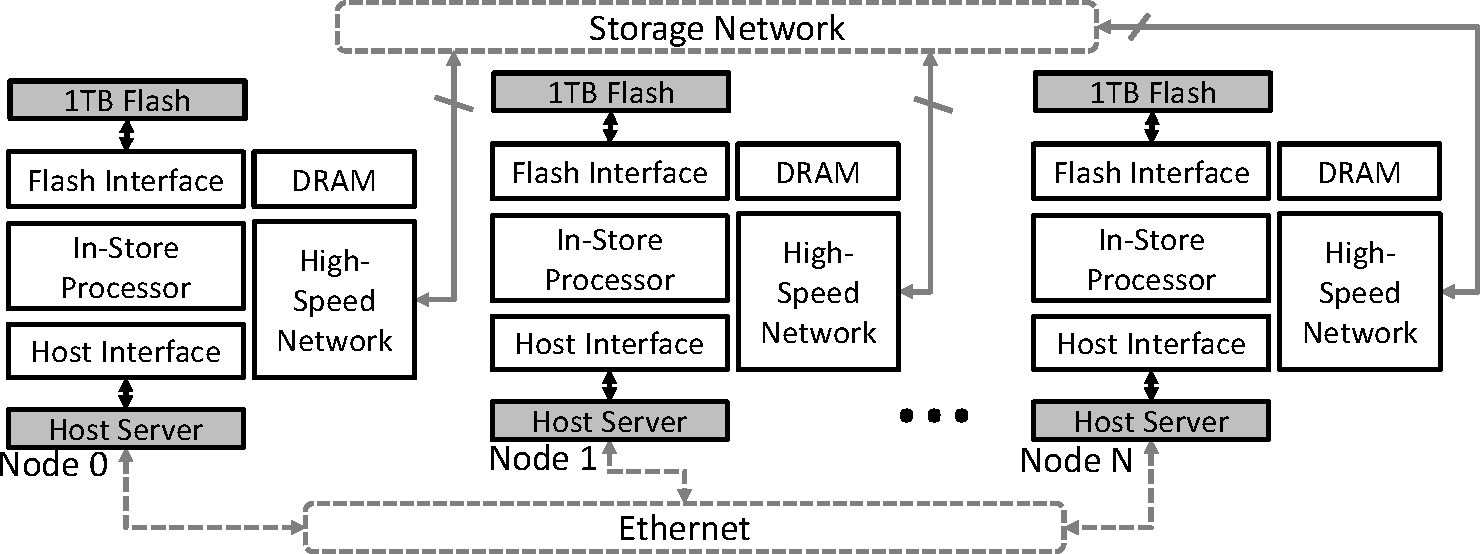
\includegraphics[width=0.8\paperwidth]{figures/architecture-crop.pdf}
	\caption{FlashBoost Architecture}
	\label{fig:architecture}
	\end{center}
\end{figure*}





\section{Related Work}
\label{sec:related}

%Modern analytics systems are usually built as a cluster of homogeneous machines
%networked using a fast interconnect. In such a configuration, the system can
%perform at its full potential if the dataset can fit in its collective DRAM.

In Big Data scale workloads, building a cluster with enough DRAM capacity to
accommodate the entire dataset can be very desirable but expensive. An example
of such a system is RAMCloud, which is a DRAM-based storage for large-scale
datacenter applications~\cite{ramcloud, rumble_log_dram}.  RAMCloud provides more than 64TBs of DRAM
storage distributed across over 1000 servers networked over high-speed
interconnect. Although RAMCloud provides 100 to 1000 times better performance
than disk-based systems of similar scale, its high energy consumption and high
price per GB limits its widespread use except for extremely performance and
latency sensitive workloads.

NAND-Flash-based SSD devices are gaining traction as a faster alternative to
disks, and close the performance gap between DRAM and persistent storage.
SSDs have the benefit of an order of magnitude cheaper price compared to DRAM,
and an order of magnitude faster performance compared to disk.
Many existing database and analytics softwares have been demonstrated to have
improved performance with SSDs~\cite{hadoopperf,ssdhadoop,ssddatabase}.
Several SSD-optimized analytics softwares, such as the SanDisk
Zetascale~\cite{zetascale} have demonstrated promising
performance while using SSD has the primary data storage.
Many commercial SSD devices have adopted high-performance PCIe interface in
order to overcome the slower SATA bus interface designed for
disk~\cite{fusionio, violinmemory, intelnvme}. Attempts to
use flash as a persistent DRAM alternative by plugging it into a RAM slot
are being explored as well~\cite{diablotechnology}. 

SSD storage devices have been largely developed to be a faster drop-in
replacement for disk drives. This backwards compatibility helped them gain
widespread adoption.  However, this required additional software and hardware to
hide the difference in device characteristics~\cite{ssddesigntradeoff}.  Due to the high performance of
SSDs, even inefficiencies in the storage management software becomes
significant, and optimizing such software has been under active investigation.
Moneta~\cite{ucsd_moneta} modifies the operating system's storage management
components to reduce software overhead when accessing NVM storage devices.
Willow~\cite{ucsd_willow} provides an easy way to augment SSD controllers with
additional interface semantics that make better use of SSD characteristics, in
addition to a backwards compatible storage interface.  Attempts to remove the
translation layers and let the databse make high-level decisions~\cite{noftl}
have shown to be beneficial. 

Another important attempt to accelerate SSD storage performance is in-storage
processing, where some data analytics is offloaded to embedded processors inside
SSDs. These processors have extremely low-latency access to storage, and helped
overcome the limitations of the storage interface bus. The idea of in-storage
processing itself is not new. The idea of intelligent disks (IDISK) connected to
each other using serial networks have been proposed in 1998~\cite{idisk}, and
adding processor to disk heads to do simple filters have been suggested as early
as in the 1970s~\cite{searchprocessor,RAP,dbc}. However, performance improvements of such special
purpose hardware did not justify their price at the time. This idea is seeing
new light with advancement of fast flash devices. This idea is seeing new light
with the advancement of fast flash technology. Devices such as Smart
SSDS~\cite{smartssdquery,smartssdcost,ucsd_willow} and Programmable
SSDs~\cite{xsd} have been investigated and showed promising results. Because of
the limited performance of embedded processors on such power-constrained
devices, embedding reconfigurable hardware on storage devices are being
investigated as well. Ibex~\cite{ibex} is a MySQL accelerator platform where a
SATA SSD is coupled with an FPGA. Relational operators such as selection and
group-by are performed on the FPGA whenever possible, otherwise they are
forwarded to software. On the other end of the spectrum, systems such as
XSD~\cite{xsd} embeds a GPU into a SSD controller, and demonstrates high
performance accelerating MapReduce.

Due to their high performance, SSDs also effect the network requirements.  The
latency to access disk over Ethernet was dominated by the disk seek latency.
However, in a SSD-based cluster the storage access latency could even be lower
than network access. These concerns are being addressed by faster network
fabrics such as 10GbE and Infiniband~\cite{infiniband}, and by low-overhead
software protocols such as RDMA~\cite{rdmampi, rdmahdfs, homrmapreduce, rdmahpc,
rdmampi, hadoopinfiniband} or user-level TCP stacks that bypass the operating
system~\cite{usertcp,userlevelprotocol}. QuickSAN~\cite{ucsd_quicksan} is an
attempt to remove a layer of software overhead by augmenting the storage device
with a low-latency NIC, so that remote storage access does not need to go
through a separate network software stack.


Building specialized hardware for databases have been extensively studied and
productized. Companies such as Oracle~\cite{exadata} and
IBM/Netezza~\cite{netezza} have used FPGAs to offload database queries.
FPGAs have been used to accelerate operations such as hash index
lookups~\cite{walkers}. Domain-specific processors for database queries are
being developed~\cite{databasefpga, hybridsql}, including Q100~\cite{q100} and LINQits~\cite{linqits}.
Q100 is a data-flow style processor with an instruction set architecture that
supported SQL queries. LINQits mapped a query language called LINQ to a set of
accelerated hardware templates on a heterogeneous SoC (FPGA + ARM). Both designs
exhibited order of magnitude performance gains at lower power, affirming that
specialized hardware for data processing is very advantageous.
%However, in both cases, experiments were
%conducted with data that is on-chip or in DRAM.
Some database accelerators benefit from being on the datapath of normal data
movement. Accelerators have been place in-path to perform low-latency operations
at wire speed~\cite{fpgastreamquery}, or to collect information such as
histogram tables~\cite{histogramssideeffect}.

\begin{figure*}[t!]
\centering
\vspace{0pt}
\begin{minipage}[c]{.4\paperwidth}
\begin{center}
	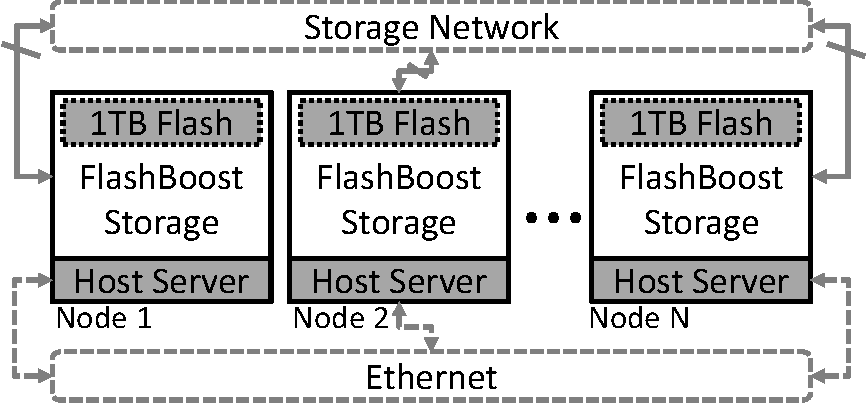
\includegraphics[width=\textwidth]{figures/architecture_small-crop.pdf}
	\caption{FlashBoost Overall Architecture}
	\label{fig:architecture}
\end{center}
\end{minipage}\hfill
\vspace{0pt}
\begin{minipage}[c]{.4\paperwidth}
\begin{center}
	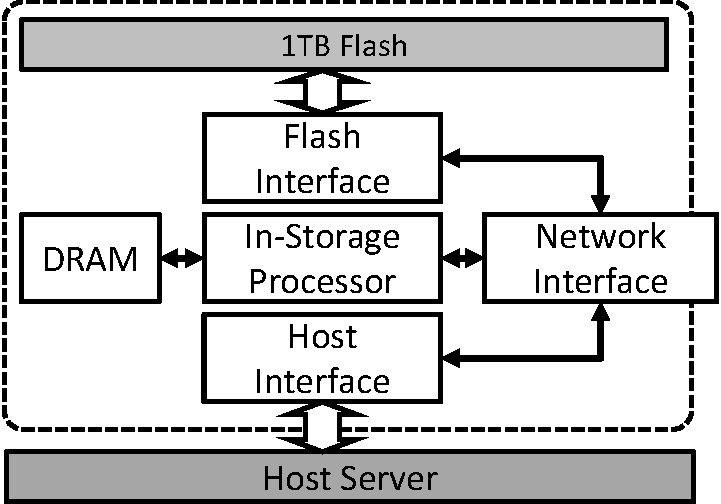
\includegraphics[width=0.7\textwidth]{figures/architecture_node-crop.pdf}
	\caption{FlashBoost Node Architecture}
	\label{fig:architecture_node}
\end{center}
\end{minipage}
\end{figure*}



Incorporating reconfigurable hardware accelerators into large datacenters are
being actively investigates as well. Microsoft recently has built and
demonstrated the power/performance benefits of a FPGA-based system called
Catapult~\cite{msr_catapult}.  Catapult uses a large number of homogeneous
servers each augmented with an FPGA.  The FPGAs form a network among themselves
via high-speed serial links so that large jobs can be mapped to groups of FPGAs.
Catapult was demonstrated to deliver much faster performance while consuming
less power, compared to a normal ram cloud cluster. FlashBoost has similar
goals in terms of reconfigurable hardware acceleration, but it uses flash
devices to accelerate lower cost systems that do not have enough collective DRAM
to host the entire dataset.

FlashBoost incorporates ideas such as in-storage processing and integrated
networks to construct a high-performance flash-based analytics appliance.
Previous work such as BlueDBM~\cite{bluedbm} have included similar features, but
FlashBoost differs in the sense that it has enough capacity to explore
real-world Big Data applications.

\section{System Architecture}
\label{sec:architecture}


The FlashBoost architecture is a homogeneous cluster of host servers coupled
with a FlashBoost storage device. Each FlashBoost storage device is plugged into
the host server via a PCIe link, and it consists of flash storage, an in-storage
processing engine, 8 high-speed network interfaces and on-board DRAM. The host
servers are networked together using Ethernet or other general-purpose
networking fabric. The host server can access the FlashBoost storage device via
a host interface implemented over PCIe. It can either directly communicate with
the flash interface, to treat is as a raw storage device, or with the in-store
processor to perform computation on the data.

The in-store processing engine has access to four major services: The flash
interface, network interface, host interface and the on-storage DRAM buffer.
Figure~\ref{fig:architecture_node} shows the four services available to the
in-storage processor. In the following sections we describe the flash interface,
network interface and host interface in order. We omit the DRAM buffer because
its design is very generic.

\subsection{Flash Interface}

Flash devices or SSDs achieve high bandwidth by grouping multiple flash chips
into several channels, all of which can operate in parallel. Because NAND flash
has limited program/erase cycles and frequent errors, complex flash management
algorithms are required to guarantee reliability. These include wear leveling,
garbage collection, bit error correction and bad block management. These
functions are typically handled by multiple ARM-based cores in the SSD
controller. The host side interface of an SSD is typically SATA or PCIe, using
AHCI or NVMe protocols to communicate with host. SSDs are viewed
as a typical block device to the host operating system, and its internal
architecture and management algorithms are completely hidden. 

However, this additional layer of management has shown to be duplicated with
file system functionalities and adds significant latency~\cite{redo}.
Furthermore, in a distributed storage environment, such as FlashBoost,
independent flash devices do not have a holistic view of the system and thus
cannot efficiently manage flash. Finally, in-store processors that we have
introduced in FlashBoost would also incur performance penalties if passing
through this extra layer. 

Thus in FlashBoost, we chose to shift flash management
away from the device and into file system/block device driver (discussed in
Section~\ref{sec:software}). Our flash controller exposes a low-level, thin,
fast and bit-error corrected hardware interface to raw NAND flash chips, buses,
blocks and pages. This has the benefit of (i) cutting down on access latency
from the network and in-store processors; (ii) exposing all degrees of
parallelism of the device and (iii) allowing higher level system stacks (file
system, database storage engine) to more intelligently manage data. 

To access the flash, the user first issues a flash command
with the operation, the address and a unique tag.
For writes, the user then awaits for a write data request from
the controller scheduler, which tells the user that the flash controller is
ready to receive the data for that write. The user will send the write data
corresponding to that request in 128-bit bursts. The controller returns an
acknowledgement once write is finished. 
For read operations, after a command is issued,
data will return in 128-bit bursts along with the command tag that the
burst corresponds to. We emphasize that for maximum performance, the
controller may send these data bursts \emph{out of order} with respect to
the issued request and \emph{interleaved} with other read requests.
Thus completion buffers may be required on the user side to maintain FIFO
characteristics. Furthermore,
we note that to saturate the bandwidth of the flash device, multiple
commands must be in-flight at the same time, since flash operations
can have latencies of 50 $\mu s$ or more. 

%Access to flash storage is provided by the flash controller via a fast,
%low-level and error-free interface with minimal overhead. This interface exposes
%the internal memory organization of the flash device, namely the buses/channels,
%chips, blocks and pages.  The interface is designed to stream data in and out of
%the flash chips as fast as possible without concern for flash management. Flash
%management functionalities such as garbage collection, bad block management and
%wear-leveling are handled by the flash-aware file system described int
%Section~\ref{sec:software}, or implemented inside the in-store processor itself.
%The key advantage of such a low-level interface is that the in-store processors
%have direct access to data with minimal overhead.

\begin{figure}[h]
	\begin{center}
	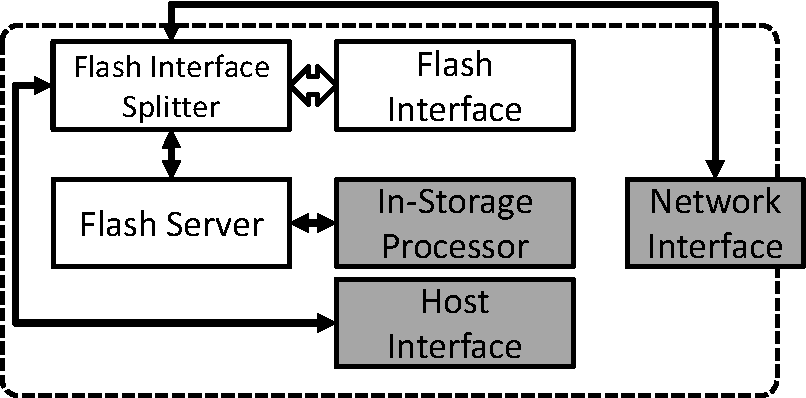
\includegraphics[scale=0.4]{figures/architecture_flash-crop.pdf}
	\caption{Flash Interface}
	\label{fig:flashinterface}
	\end{center}
\end{figure}

\subsubsection{Multiple Access Agents}

Multiple hardware endpoints in FlashBoost may need shared access to this
flash controller interface. For example, a particular controller may
be accessed by local in-store processors, local host software over PCIe
DMA, or remote in-store processors over the network. Thus we implemented a
Flash Interface Splitter with tag renaming to manage multiple users
(Figure~\ref{fig:flashinterface}). In addition, 
to ease development of hardware in-store processors,
we also provide an optional Flash Server module as part of FlashBoost. This server
converts the out-of-order and interleaved flash interface into
multiple simple in-order request/response interfaces
using page buffers. It also contains an Address Translation Unit that 
maps file handles to incoming streams of physical addresses from the host. The in-store processor
simply makes a request with the file handle, offset and length, and the Flash Server will perform
the flash operation at the corresponding physical location. The software
support for this function is discussed in Section~\ref{sec:software}). The Flash
Server's width, command queue depth and number of interfaces is adjustable 
based on the application.

\subsection{Integrated Storage Network}

\begin{figure}[t]
	\begin{center}
	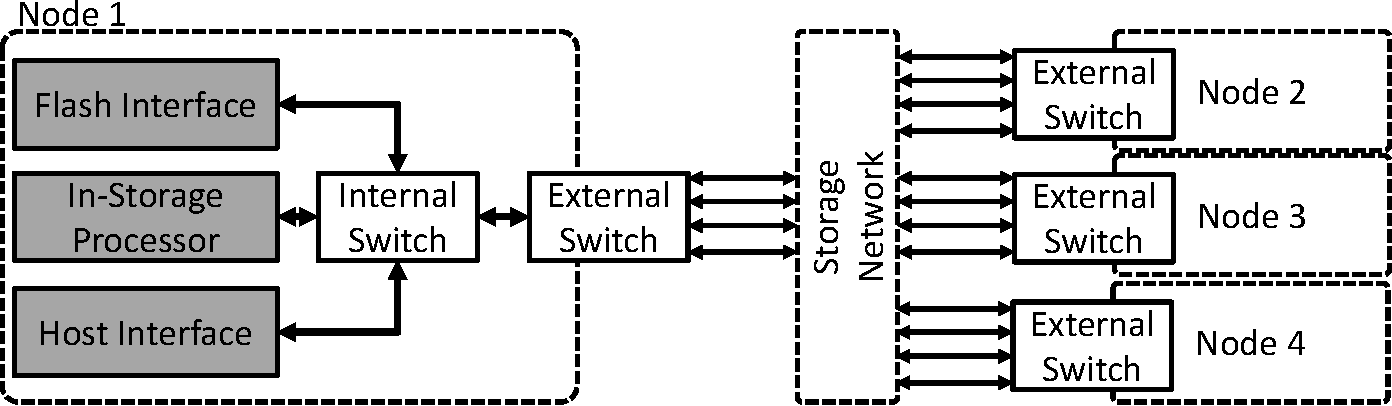
\includegraphics[width=0.5\textwidth]{figures/network-architecture-crop.pdf}
	\caption{Network Architecture}
	\label{fig:networkinterface}
	\end{center}
\end{figure}


FlashBoost provides a low-latency high-bandwidth network infrastructure across
all FlashBoost storage devices in the cluster, while maintaining a simple design
with low resource usage. FlashBoost storage devices form a separate network
among themselves via high-performance serial links.  The FlashBoost network is a
packet-switched mesh network, in which each storage device has multiple network
ports and is capable of routing packets across the network without requiring a
separate switch or router.  In addition to routing, the storage network supports functionality such as
flow control and virtual channels while maintaining high performance and
extremely low latency.  For data traffic between the storage devices, the
integrated network ports removes the overhead of going to the host software to
access a separate network interface.

Figure~\ref{fig:networkinterface} shows the network architecture. Switching is
done at two levels, the internal switch and the external switch.  The internal
switch routes packets between local components.  The external switch accesses
multiple physical network ports, and is responsible for relaying data from a
port to another port in order to relay a packet to its next hop. It is also
responsible for relaying inbound packets to the internal
switch, and relaying outbound packets from the internal switch to a correct
physical port. 

Due to the multiple ports on the storage nodes, the FlashBoost network is very
flexible and can be configured to implement various topologies, as long as no
one node requires more connections than the number of ports on it.
Figure~\ref{fig:topologies} shows some example topologies. To implement a
different topology the physical cables between each node has to be re-wired, but
the routing across a topology can be configured dynamically by the software.

%Components that want to use the network choose one or more \emph{Logical
%Endpoints}, which provide virtual channel semantics, to access the network in a
%virtualized manner.

\begin{figure}[t!]
	\centering
	\subfloat[Distributed Star]
		{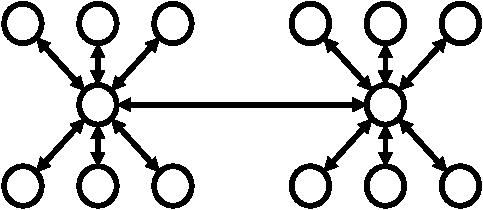
\includegraphics[scale=0.35]{figures/topology_dist_star-crop.pdf}}
		\hfill
	\subfloat[Mesh]
		{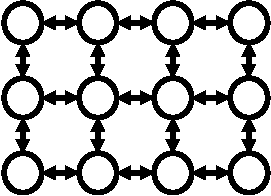
\includegraphics[scale=0.35]{figures/topology_mesh-crop.pdf}}
		\hfill
	\subfloat[Fat Tree]
		{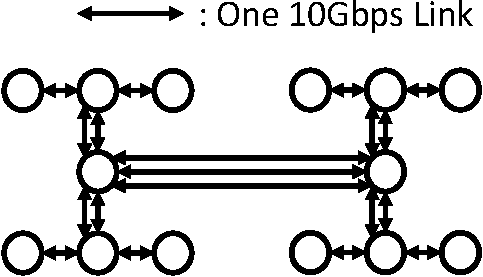
\includegraphics[scale=0.35]{figures/topology_fat_tree-crop.pdf}}
	\caption{Any Network Topology Is Possible As Long As It Requires Less Than 8
	Network Ports Per Node}
	\label{fig:topologies}
\end{figure}


\subsubsection{Logical Endpoint}

The FlashBoost network infrastructure exposes virtual channel semantics to the
users of the network by providing it with multiple \emph{logical endpoints}.  The
number of endpoints are determined at design time by setting a parameter, and
all endpoints share the physical network.  Each endpoint is parameterized with a
unique index that does not need to be contiguous.  Each endpoint exposes two
interfaces, \texttt{send} and \texttt{receive}. An in-storage processor can send
data to a remote node by calling \texttt{send} with a pair of data and
destination node index, or receive data from remote nodes by calling
\texttt{receive}, which returns a pair of data and source node index. These
interfaces provide back pressure, so that each endpoint can be treated like a
FIFO interface across the whole cluster. Such intuitive characteristics of the
network ease development of in-storage processors.

\subsubsection{Link Layer}

The link layer manages physical connections between network ports in the storage
nodes. The most important aspect of the link layer is the simple token-based
flow control implementation. This provides back pressure across the link and
assures that no packet will drop if the data rate is higher than what the
network can manage, or if the data is not received from the destination node
quick enough.

\subsubsection{Routing Layer}

%The goals of the FlashBoost network infrastructure is to
%maintain high bandwidth and low latency, while maintaining a simple design for
%embedded implementation. This requirement
%prompted many design choices.

\begin{figure}[h]
	\begin{center}
	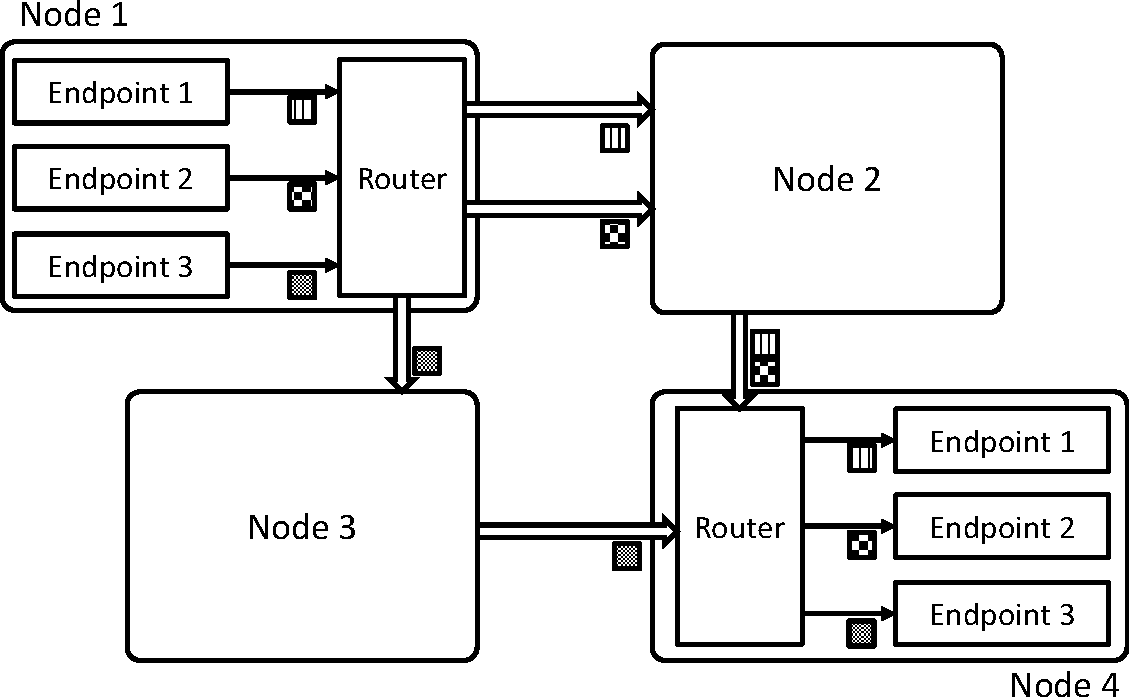
\includegraphics[width=0.4\textwidth]{figures/routing-crop.pdf}
	\caption{Routing Packets Across the Network}
	\label{fig:networkrouting}
	\end{center}
\end{figure}

In order to make maximum use of the bandwidth of the network infrastructure
while keeping resource usage to a minimal, the FlashBoost network implements
deterministic routing for each logical endpoint. This means that all packets
originating from the same logical endpoint that are directed to the same
destination node follow the same route across the network, while packets from a
different endpoint directed to the same destination node may follow a different
path. Figure~\ref{fig:networkrouting} shows packet routing in an example
network. The benefits of this approach is that packet traffic can be distributed
across multiple links, while maintaining the order of all packets from the same
endpoint. If packets from the same endpoint are allowed to take different paths,
it would require a completion buffer which may be expensive in an embedded
system.
For simplicity, the FlashBoost network does not implement a discovery protocol, and relies on a
network configuration file to populate the routing tables. 

In order to maintain extremely low network latency, each endpoint is given a
choice whether to use end-to-end flow control or not. If the developer is sure
that a particular virtual link will always drain on the receiving end, flow
end-to-end flow control can be omitted for that endpoint. However, if the
receiver fails to drain data for a long time, the link-level back pressure may
cause related parts of the network to block. On the other hand, an endpoint can
be configured to only send data when there is space on the destination endpoint,
which will assure safety but result in higher latency due to flow control
packets, and more memory usage for buffers.

\subsection{Host Interface}

The in-storage processing core can be accessed from the host server over either
a direct interface that supports RPC and DMA operations, or a file system
abstraction built on top of the direct interface. The file system interface is
described in detail in Section~\ref{sec:software}.

In order to parallelize requests and maintain high performance, the host
interface provides the software with 128 page buffers, each for reads and
writes. When writing a page, the software will request a free write buffer, copy
data to the write buffer, and send a write request over RPC with the
physical address of the destination flash page.
The buffer will be returned to the free queue when the
hardware has finished reading the data from the buffer. When reading a page, the
software will request a free read buffer, and send a read request over RPC with
the physical address of the source flash page. The software will receive an
interrupt with the buffer index when the hardware has finished writing to
software memory.

Using DMA to write data to the storage device is straightforward to parallelize,
but parallelizing reads is a bit more tricky due to the characteristics of flash
storage. When writing to storage, the DMA engine on the hardware will read data
from each buffer in order in a contiguous stream. So having enough requests in
the request queue is enough to make maximum use of the host-side link bandwidth.
However, data read from flash chips on multiple buses in parallel can arrive
interleaved at the DMA engine. Because the DMA engine needs to have enough
contiguous data for a DMA burst before issuing a DMA burst, some reordering may
be required at the DMA engine. This becomes even more tricky when the device is
using the integrated network to receive data from remote nodes, where they might
all be coming from different buses. To fix this issue, we provide dual-ported
buffer in hardware providing the semantics of a vector of FIFOs, so that data
for each request can be enqueued into its own FIFO until there is enough data
for a burst.
Figure~\ref{fig:hostinterface} describes the structure of the host interface for
flash reads.

\begin{figure}[t!]
	\centering
	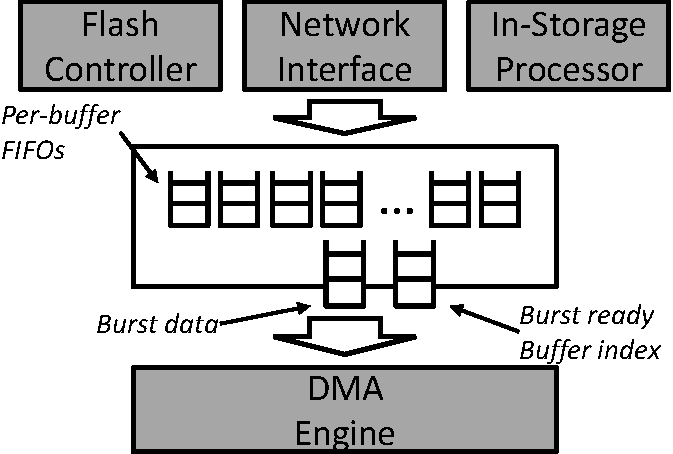
\includegraphics[width=0.3\textwidth]{figures/dmawrite-crop.pdf}
	\caption{Host-FPGA Interface Over PCIe}
	\label{fig:hostinterface}
\end{figure}

%TODO: \subsubsection{Storage Bridge to Host}


%%%% Comments!

\begin{comment}
The raw flash interface, in hardware, is defined below:

%[captionpos=b, caption={Flash Controller Interface}, label={lst:hwifc}]
\begin{lstlisting}
interface FlashIfc;       
  method sendCmd (FlashOp op, Bit#(4) bus,
                  Bit#(3) chip, Bit#(16) block, 
                  Bit#(8) page, Bit#(8) tag);        
  method writeWord (Bit#(128) data, Bit#(8) tag);
  method Tuple2#(Bit#(128), Bit#(8)) readWord (); 
  method Bit#(8) writeDataReq ();
  method Tuple2#(Bit#(8), StatusT) ackStatus ();
endinterface 
\end{lstlisting}
\end{comment}



\begin{figure}[h]
	\begin{center}
	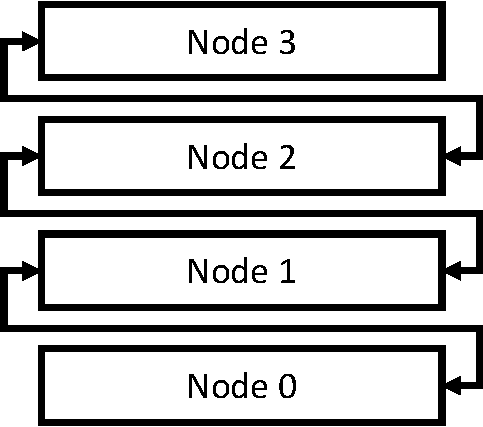
\includegraphics[width=0.15\textwidth]{resources/topology-crop.pdf}
	\caption{Prototype Topology}
	\label{fig:topology}
	\end{center}
\end{figure}

\section{Implementation Details}
\label{sec:implementation}

We have implemented a prototype of the network described using a cluster
machines. Each node in the cluster consists of one Intel Xeon-based server,
Xilinx VC707 FPGA development board, and a network expansion card. Each VC707
development board was augmented with a network expansion card that plugged into
the FMC expansion port, which pinned out the four GTX multi-gigabit serial
transceivers assigned to the high pin count FMC port into four SATA ports. SATA
crossover cables were used to connect the network expansion cards. Two lanes, or
two SATA cables were grouped together to form a channel. In the prototype system
the cluster was networked into a one-dimensional bar topology, depicted in
Figure~\ref{fig:topology}. Since the VC707 board has two FMC ports, each node
can have a fan out of up to 4 channels, which can be used to implement other
various kinds of topologies. Any direct network with a fan-out per node of 4 or
less can be implemented. Some examples of such topologies are depicted in
Figure~\ref{fig:topologies}.


\begin{figure}[h]
	\centering
	\subfloat[Star]
		{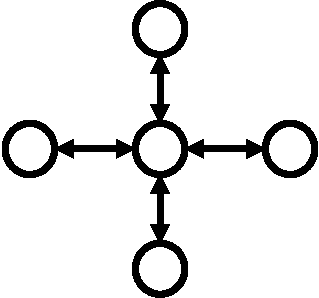
\includegraphics[scale=0.35]{resources/star-crop.pdf}}
		\hfill
	\subfloat[Tree]
		{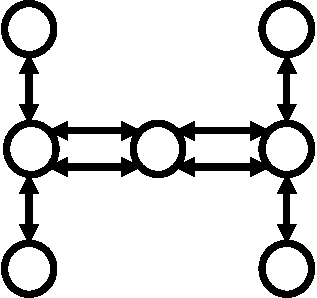
\includegraphics[scale=0.35]{resources/tree-crop.pdf}}
		\hfill
	\subfloat[Mesh]
		{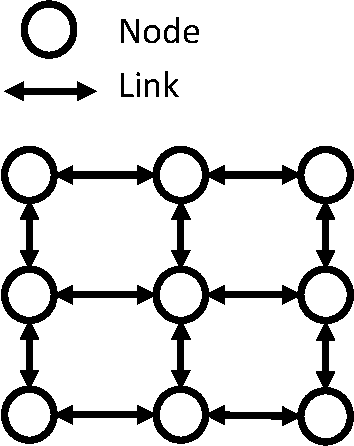
\includegraphics[scale=0.35]{resources/mesh-crop.pdf}}
	\caption{Any Network Topology With Less Than 4 Fan-Out is Possible}
	\label{fig:topologies}
\end{figure}


The link latency of an aurora link based on the GTX multi-gigabit transceiver
was measured to be around 0.48us, which translates to about 75 cycles on the
6.4ns user clock. The link layer flow control was implemented with a
conservative size of 200 beats for the round trip delay.

\subsection{FPGA Resource Utilization}

We have measured the FPGA resource utilization of our network using a simple
setup with two endpoints: one high speed endpoint with larger flow control
stride and buffer size (Stride of 200 and buffer size of 1024 packets), and one
small endpoint with smaller buffers. The endpoint row in the table below
described the larger endpoint. The router component includes the chaining logic
used to link the endpoints to it. The user logic was clocked at 125MHz.

\begin{table}[h]
	\begin{center}
	\begin{tabular}{l | c | c | }
		Component & LUTS & RAMB36 \\
		\hline
		\hline
		Aurora Link & 4843 & 36 \\
		Router & 3743 & 0 \\
		Endpoint ($\times$2) & 753 & 3 \\
		\hline
		\hline
		Total & 10092 & 42\\
		Virtex 7 Percentage   & (3\%) & (4\%) \\
	\end{tabular}
	\caption{FPGA Resource Utilization}
	\label{tab:fpgautil}
	\end{center}
\end{table}

\section{Results}
\subsection{Configurations}

\subsection{Distributed Flash Access Performance}
Latency for local flash reads, reads from local DRAM, remote reads over
fpga/serial, remote reads over serial/host DRAM, remote reads over
ethernet/Flash ethernet/DRAM

Aggregate bandwidth for flash, collecting all flash to one node, flash to pcie?

Aggregate bandwidth for competing workloads on multiple servers \(scalability\)

\subsection{Distributed Analytics Performance}

Measure latency of 8K page reads + filtering for flash, host DRAM, remote flash,
remote host DRAM, remote host DRAM with sw filtering




\section{Conclusion}
\label{sec:conclusion}

An efficient and high-performance network is essential for development of an
effective distributed FPGA computing platform. Due to high engineering cost and
the scarce on-chip memory resource, many existing inter-FPGA network
implementations do not provide transport-level network functionality such as
end-to-end flow control and virtual channels. Because such systems depend on the
user application developer to implement such features and write safe
applications, it becomes difficult to create complex distributed FPGA
applications which are also deadlock-safe and high performance.

In this paper, we have presented our design of a parameterized, low overhead
transport-layer network that provides useful features such as
virtual channels and end-to-end flow control. Our network takes advantage of the
high reliability of the high-speed serial links, which are integrated in the
FPGA fabric, to implement a lossless in-order network layer, which allowed us to
simplify the transport layer and use less FPGA resources. The design of the
transport layer is parameterized, so that the developer can choose to use less
resources while meeting the performance requirements of the individual endpoint.
Our prototype implementation demonstrated a high performance in an FPGA cluster
setting. We predict that our network will accelerate future research of
distributed FPGA applications.





% conference papers do not normally have an appendix


% use section* for acknowledgement
%\section*{Acknowledgment}
%The authors would like to thank...





% trigger a \newpage just before the given reference
% number - used to balance the columns on the last page
% adjust value as needed - may need to be readjusted if
% the document is modified later
%\IEEEtriggeratref{8}
% The "triggered" command can be changed if desired:
%\IEEEtriggercmd{\enlargethispage{-5in}}

% references section

% can use a bibliography generated by BibTeX as a .bbl file
% BibTeX documentation can be easily obtained at:
% http://www.ctan.org/tex-archive/biblio/bibtex/contrib/doc/
% The IEEEtran BibTeX style support page is at:
% http://www.michaelshell.org/tex/ieeetran/bibtex/
%\bibliographystyle{IEEEtran}
% argument is your BibTeX string definitions and bibliography database(s)
%\bibliography{IEEEabrv,../bib/paper}
%
% <OR> manually copy in the resultant .bbl file
% set second argument of \begin to the number of references
% (used to reserve space for the reference number labels box)

\bibliographystyle{IEEEtran}
\bibliography{IEEEabrv,references,network}

%\begin{thebibliography}{1}
%
%\bibitem{IEEEhowto:kopka}
%H.~Kopka and P.~W. Daly, \emph{A Guide to \LaTeX}, 3rd~ed.\hskip 1em plus
%  0.5em minus 0.4em\relax Harlow, England: Addison-Wesley, 1999.
%
%\end{thebibliography}




% that's all folks
\end{document}


